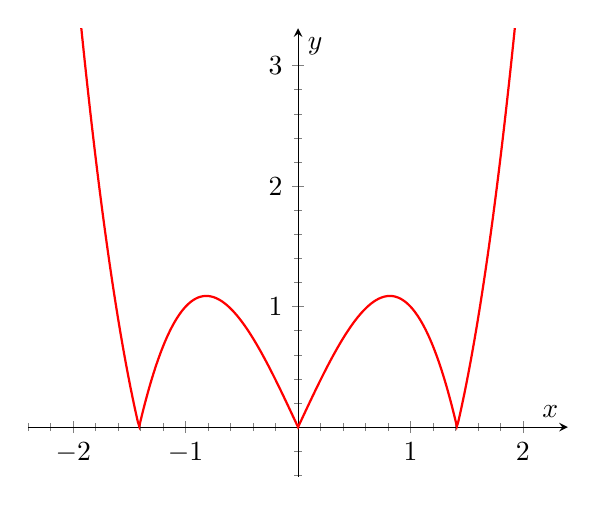
\begin{tikzpicture}[
  dfeil/.style={shorten <=1mm,>=latex,->},
 ifeil/.style={shorten <=1mm,>=latex,<-},
bfeil/.style={shorten <=1mm,>=latex,<->},
]
\begin{axis}[
        axis x line=middle,
        axis y line=middle,
        minor tick num=4,
        %width=9cm,
        %height=4.5cm,
        xmin=-2,     % start the diagram at this x-coordinate
        xmax= 2,    % end   the diagram at this x-coordinate
        ymin=-0.1,     % start the diagram at this y-coordinate
        ymax= 3,   % end   the diagram at this y-coordinate
        xlabel=$x$,
        ylabel=$y$,
     % ticks=none,
        enlargelimits=true,
        ]
\addplot[thick,bfeil,domain=-2.5:2.5,samples=401,red] {abs(x^3 - 2*x)};
\end{axis}
\end{tikzpicture}